\input{/Users/Martin/Documents/Documents/gitRepo/Scripts/Latex/templates/beamerTemplate}
% Material Derivative Eq. - Vector notation 
\newcommand{\materialDerivativeVec}[1] %\materialDerivativeVec{\rho V}
{   \frac{D}{Dt}\B(#1\E) = \frac{\partial}{\partial t}\B(#1\E) + \B(\vec{V}\cdot\nabla\E) #1   }

% Reynolds Transport Theorem 
\newcommand{\reynoldsTransportTheorem}[1] %\reynoldsTransportTheorem{\vec{F}} 
{ \frac{D}{Dt}\int_{C\forall}#1d\forall = \int_{C\forall}\PartialFrac{#1}{t}d\forall + \oint_{CS} \Parenthesis{ \Sub{\vec{V}}{relative} \cdot \hat{n} }#1dS }

% Continuity Eq. 
\newcommand{\continuityVec}
{   \dot{\rho} + \nabla\cdot\Parenthesis{ \rho\vec{V} }   }

% Continuity Eq. - Cartesian coordinates  
\newcommand{\continuityCartesian} %continuityEqExpanded (former name)
{ \dot{\rho} + \PartialFrac{\Parenthesis{\rho u}}{x} + \PartialFrac{\Parenthesis{ \rho v}}{y} + \PartialFrac{\Parenthesis{\rho w}}{z} }

% Continuity Eq. - Cylindrical coordinates 
\newcommand{\continuityCylindrical} 
{ \dot{\rho} + \frac{1}{r}\PartialFrac{ }{r}\Parenthesis{ \rho r\Sub{v}{r} } + \frac{1}{r}\PartialFrac{ }{\theta}\Parenthesis{\rho\Sub{v}{\theta}} + \PartialFrac{ }{z}\Parenthesis{\rho\Sub{v}{z}} }

% Continuity Eq. - Spherical coordinates 
\newcommand{\continuitySpherical} 
{ \dot{\rho} + \frac{1}{r^2}\PartialFrac{}{r}\Parenthesis{ \rho r^2\Sub{v}{r} } + \frac{1}{ r\sin(\theta) }\PartialFrac{}{\theta}\Parenthesis{ \rho\sin(\theta)\Sub{v}{\theta} } + \frac{1}{ r\sin(\theta) }\PartialFrac{}{\phi}\Parenthesis{ \rho\Sub{v}{\phi} } }

% Incompressible Navier Stokes Eq - Material derivative 
\newcommand{\incompressibleNavierStokesMaterial} 
{ \rho\frac{D\vec{V}}{Dt} = -\nabla P + \mu \Up{\nabla}{2}V + \Sub{B}{f} }

% Incompressible Navier Stokes Eq. - Vector notation  
\newcommand{\incompressibleNavierStokesVec} 
{   \rho\Parenthesis{ \dot{V} + \Parenthesis{\vec{V}\cdot\nabla}V } = -\nabla P + \mu \Up{\nabla}{2}V + \Sub{B}{f}  }

% Incompressible Navier Stokes Eq. - Vector expanded
\newcommand{\incompressibleNavierStokesCartesian}[2] %\incompressibleNavierStokesExpanded %\incompressibleNavierStokesCartesian{u}{x}
{ \rho\Parenthesis{ \dot{#1} + u\PartialFrac{#1}{x} + v\PartialFrac{#1}{y} + w\PartialFrac{#1}{z} } = -\PartialFrac{P}{#2} + \mu\Parenthesis{ \PartialFracN{#1}{x}{2} + \PartialFracN{#1}{y}{2} + \PartialFracN{#1}{z}{2} } + \Sub{f}{#2} }

% Incompressible Navier Stokes Eq. - Cylindrical on r direction 
\newcommand{\incompressibleNavierStokesCylindricalR} 
{ \rho\Parenthesis{ \Sub{\dot{v}}{r} + \Sub{v}{r}\PartialFrac{\Sub{v}{r}}{r} + \frac{\Sub{v}{\theta}}{r}\PartialFrac{\Sub{v}{r}}{\theta} -\frac{\Sub{v}{\theta}^2 }{r} + \Sub{v}{z}\PartialFrac{\Sub{v}{r}}{z}}  =   - \PartialFrac{P}{r}  + \mu\Parenthesis{ \frac{1}{r}\PartialFrac{}{r}\Parenthesis{r\PartialFrac{\Sub{v}{r}}{r} } -\frac{\Sub{v}{r}}{r^2}  + \frac{1}{r^2}\PartialFracN{\Sub{v}{r}}{\theta}{2} - \frac{2}{r^2}\PartialFrac{\Sub{v}{r}}{\theta} +  \PartialFracN{\Sub{v}{r}}{z}{2}  } + \Sub{f}{r} }

% Incompressible Navier Stokes Eq. - Cylindrical on theta direction 
\newcommand{\incompressibleNavierStokesCylindricalTheta} 
{ \rho\Parenthesis{ \Sub{\dot{v}}{\theta} + \Sub{v}{r}\PartialFrac{\Sub{v}{\theta}}{r} + \frac{\Sub{v}{\theta}}{r}\PartialFrac{\Sub{v}{\theta}}{\theta} + \frac{\Sub{v}{r}\Sub{v}{\theta}}{r} + \Sub{v}{z}\PartialFrac{\Sub{v}{\theta}}{z}}  = - \frac{1}{r}\PartialFrac{P}{\theta} + \mu\Parenthesis{  \frac{1}{r}\PartialFrac{}{r}\Parenthesis{r\PartialFrac{\Sub{v}{\theta}}{r} } - \frac{\Sub{v}{\theta}}{r^2}  +  \frac{1}{r^2}\PartialFracN{\Sub{v}{\theta}}{\theta}{2} + \frac{2}{r^2}\PartialFrac{\Sub{v}{r}}{\theta} + \PartialFracN{\Sub{v}{\theta}}{z}{2}  } + \Sub{f}{\theta} } 

% Incompressible Navier Stokes Eq. - Cylindrical on z direction 
\newcommand{\incompressibleNavierStokesCylindricalZ} 
{  \rho\Parenthesis{ \Sub{\dot{v}}{z} + \Sub{v}{r}\PartialFrac{\Sub{v}{z}}{r} + \frac{\Sub{v}{\theta}}{r}\PartialFrac{\Sub{v}{z}}{\theta} + \Sub{v}{z}\PartialFrac{\Sub{v}{z}}{z} } = -\PartialFrac{P}{z} + \mu\Parenthesis{ \frac{1}{r}\PartialFrac{ }{r}\Parenthesis{r\PartialFrac{\Sub{v}{z}}{r}} + \frac{1}{r^2}\PartialFracN{\Sub{v}{z}}{\theta}{2} + \PartialFracN{\Sub{v}{z}}{z}{2} }+\Sub{f}{z}  } 

% Incompressible Navier Stokes Eq. - Einstein's notation  
\newcommand{\incompressibleNavierStokesEins}
{   \rho\Parenthesis{ \Sub{\dot{V}}{k} + \Sub{V}{i}\Partial{j}\Sub{V}{k}\Sub{\delta}{ij} } = -\Partial{k}P + \mu\UpSub{\partial}{j}{2}\Sub{V}{k} + \Sub{f}{k}   }

% Non-dimensional Navier Stokes Eq. 
\newcommand{\nonDimensionalNavierStokes} 
{\SqBracket{St}\frac{D\vec{V}^*}{Dt^*} = -\SqBracket{Eu}\nabla^*P^*  +\SqBracket{\frac{1}{Re}}\nabla^{*^{2}}V^* + \SqBracket{\frac{1}{Fr^2}}g^* }

% Shear Strain Tensor 
\newcommand{\shearStrainTensor}
{ \Sub{\varepsilon}{ij} = \frac{1}{2}\Parenthesis{ \PartialFrac{\Sub{v}{i}}{\Sub{x}{j}} + \PartialFrac{\Sub{v}{j}}{\Sub{x}{i}} } }

% Shear Stress Tensor, Stokes Hypothesis is assumed  
\newcommand{\shearStressTensor} 
{ \Sub{\tau}{ij} = 2\mu\SqBracket{ \Sub{\varepsilon}{ij} -\frac{1}{3} \Parenthesis{ \PartialFrac{\Sub{v}{k}}{\Sub{x}{k}}  }\Sub{\delta}{ij} }} 

% Total Stress Tensor (Cauchy Momentum Tensor) 
\newcommand{\cauchyMomentumTensor} %totalStressTensor 
{ \Sub{\sigma}{ij} = -p\Sub{\delta}{ij} + \Sub{\tau}{ij} }

% Gradient operator - Cartesian coordinates 
\newcommand{\gradientCartesian}[1] %\gradientCartesian{v}
{ \PartialFrac{#1}{x}\hat{x} + \PartialFrac{#1}{y}\hat{y} + \PartialFrac{#1}{z}\hat{z} }

% Divergence operator - Cartesian coordinates 
\newcommand{\divergenceCartesian}[3] %\diverganceCartesian{u}{v}{w} 
{ \PartialFrac{#1}{x} + \PartialFrac{#2}{y} + \PartialFrac{#3}{z} }

% Laplace operator - Cartesian coordinates 
\newcommand{\laplaceCartesian}[1] %\laplaceCartesian{u}
{ \PartialFracN{#1}{x}{2} + \PartialFracN{#1}{y}{2} + \PartialFracN{#1}{z}{2} }

% Gradient operator - Cylindrical coordinates  
\newcommand{\gradientCylindrical}[1] %\gradientCylindrical{f} 
{ \PartialFrac{#1}{r}\hat{r} + \frac{1}{r}\PartialFrac{#1}{\theta}\hat{\theta} + \PartialFrac{#1}{z}\hat{z} }

% Divergence operator - Cylindrical 
\newcommand{\divergenceCylindrical}[3] %\divergenceCylindrical{r}{\theta}{a} 
{ \frac{1}{r}\PartialFrac{\Parenthesis{r#1}}{r} + \frac{1}{r}\PartialFrac{#2}{\theta} + \PartialFrac{#3}{z} }

% Laplace operator - Cylindrical coordinates 
\newcommand{\laplaceCylindrical}[1] %\laplaceCylindrical{V} 
{ \frac{1}{r}\PartialFrac{ }{r}\Parenthesis{r\PartialFrac{#1}{r}} + \frac{1}{r^2}\PartialFracN{#1}{\theta}{2} + \PartialFracN{#1}{z}{2} }

% Gradient operator - Spherical coordinates 
\newcommand{\gradientSpherical}[1] %\gradientSpherical{V}  
{ \PartialFrac{#1}{r}\hat{r} + \frac{1}{r}\PartialFrac{#1}{\theta}\hat{\theta} + \frac{1}{r\sin\Parenthesis{\theta}}\PartialFrac{#1}{\phi}\hat{\phi} }

% Divergence operator - Spherical coordinates 
\newcommand{\divergenceSpherical}[3] %\divergenceSpherical{r}{\theta}{\phi} 
{ \frac{1}{r^2}\PartialFrac{\Parenthesis{r^2#1}}{r} + \frac{1}{r\sin\Parenthesis{\theta}}\PartialFrac{}{\theta}\SqBracket{#2\sin\Parenthesis{\theta}} + \frac{1}{r\sin\Parenthesis{\theta}}\PartialFrac{#3}{\phi} }

% Laplace operator - Spherical coordinates 
\newcommand{\laplaceSpherical}[1] %laplaceSpherical{f} 
{ \frac{1}{r^2}\PartialFrac{}{r}\Parenthesis{r^2\PartialFrac{#1}{r}} + \frac{1}{r^2\sin\Parenthesis{\theta}}\PartialFrac{}{\theta}\Parenthesis{\sin\Parenthesis{\theta}\PartialFrac{#1}{\theta}} + \frac{1}{r^2\sin\Parenthesis{\theta}}\PartialFracN{#1}{\phi}{2} }

% Dot Product - Einstein's notation 
\newcommand{\dotEins}[4] %\dotEins{A}{i}{B}{j} 
{ \Sub{#1}{#2}\Sub{#3}{#4}\Sub{\delta}{#2#4} }

% Cross Product - Einstein's notation 
\newcommand{\crossEins}[5] %\crossEins{ijk}{A}{i}{B}{k}  
{ \Sub{\varepsilon}{#1}\Sub{#2}{#3}\Sub{#4}{#5} }

% Stokes Theorem 
\newcommand{\stokesTheorem}[1] %\stokesTheorem{F} 
{ \Sub{\oint}{C}{#1}\cdot d\vec{r} = \iint\Parenthesis{\nabla\times {#1} }\cdot\,d\vec{S} }

% Divergence Theorem 
\newcommand{\divergenceTheorem}[1] %\divergenceTheorem{F}
{ \Sub{\iiint}{\forall}\Parenthesis{\nabla\cdot #1}d\forall = \Sub{\oiint}{S}\Parenthesis{#1\cdot\hat{n}}dS } 

%  Leibniz Integral Rule
\newcommand{\leibnizIntegral} 
{ \frac{d}{dx}\int^{b}_{a}\Function{f}{x,t}dt = \SqBracket{ \Function{f}{x,b}\PartialFrac{b}{x} - \Function{f}{x,a}\PartialFrac{a}{x} } + \int^{b}_{a}\PartialFrac{ }{x} \Function{f}{x,t}dt }  

% Taylor Series 
\newcommand{\taylorSeries} 
{ \sum_{n=1}^{\infty}\frac{f^{(n)}(a)}{n!}\B(x-a\E)^n }

% Maxwell Equations - Differential notation 
\newcommand{\maxwellEqA}
{   \nabla\cdot\bm{E}  = \frac{\rho}{\Sub{\varepsilon}{0}}  } 
\newcommand{\maxwellEqB} 
{   \nabla\cdot\bm{B} = 0   } 
\newcommand{\maxwellEqC} 
{   \nabla\times\bm{E} = - \frac{\partial\bm{B}}{\partial t}    }
\newcommand{\maxwellEqD} 
{   \nabla\times\bm{B} = \Sub{\mu}{0}\bm{j} + \frac{1}{\Up{c}{2}}\frac{\partial\bm{E}}{\partial t}  }

% Quadratic equation 
\newcommand{\quadraticEq}[3] %\quadratic{a}{b}{c} 
{ \frac{  -(#2) \pm \sqrt{ (#2)^2 - 4(#1) (#3) } }{2(#1)} }

% Binomial coeficient 
\newcommand{\binomialCoeff} 
{ \binom{n}{k} = \frac{n!}{k!\Parenthesis{n-k}!} } 




%Rename math commands
\everymath{\displaystyle} %display style for everymath 
\newcommand{\B}{\left}	  
\newcommand{\E}{\right}
\newcommand{\Acronym}[2]{\B( #1_{_{#2}}\E)}
\newcommand{\Avg}[1]{\langle#1\rangle}
\newcommand{\Parenthesis}[1]{\B(#1\E)}
\newcommand{\SqBracket}[1]{\B[#1\E]}
\newcommand{\Sub}[2]{#1_{_{#2}}} 
\newcommand{\Up}[2]{#1^{^{#2}}} 
\newcommand{\UpSub}[3]{#1_{_{#2}}^{^{#3}}}
\newcommand{\Result}[1]{\bm{\boxed{#1}}}
\newcommand{\Limit}[2]{\underset{#1\rightarrow#2}{\lim}} 
\newcommand{\Function}[2]{#1_{\Parenthesis{#2}}} 
\newcommand{\Units}[1]{\,\SqBracket{#1}} 
\newcommand{\UnitsFrac}[2]{\,\SqBracket{\frac{#1}{#2}}} 
\newcommand{\Abs}[1]{\B\lvert#1\E\rvert} 
\newcommand{\Norm}[1]{\B\lVert#1\E\rVert} 

% Derivatives 
\newcommand{\Partial}[1]{\Sub{\partial}{#1}} 
\newcommand{\PartialFrac}[2]{\frac{\partial #1}{\partial #2}} 
\newcommand{\PartialFracN}[3]{\frac {\Up{\partial}{#3} #1}{\partial \Up{#2}{#3}}} 
\newcommand{\PartialDer}[2]{\frac{\partial #1}{\partial #2}} 
\newcommand{\PartialDerN}[3]{\frac {\Up{\partial}{#3} #1}{\partial \Up{#2}{#3}}} 
\newcommand{\TotalDer}[2]{\frac{d #1}{d #2}} 

% Trig  
\newcommand{\Sin}[1]{\sin\Parenthesis{#1}}
\newcommand{\SinFrac}[3]{\sin\Parenthesis{ \frac{#1}{#3} #2}}
\newcommand{\Cos}[1]{\cos\Parenthesis{#1}}
\newcommand{\CosFrac}[3]{\cos\Parenthesis{ \frac{#1}{#3} #2}}
\newcommand{\Tan}[1]{\tan\Parenthesis{#1}}
\newcommand{\TanFrac}[3]{\tan\Parenthesis{ \frac{#1}{#3} #2}}
\newcommand{\Ln}[1]{\ln\B|\E|}
\newcommand{\LnFrac}[2]{\ln\B|\frac{#1}{#2}\E|}

%Beamer Macro 
%\textPicture{frameTitle}{text}{pictureHeigh}{pictureName} 
\newcommand{\textPicture}[4]
{ 
	\begin{frame}{#1} 
		\vspace{-1.5cm}
		\begin{columns}[T] 
			%Insert Text 
			\begin{column}[T]{5cm}
				{#2} 
			\end{column}
		
			%Insert Picture 
			\begin{column}[T]{4cm} 
				\includegraphics[height=#3cm]{#4} 
			\end{column} 
		\end{columns} 
	\end{frame} 
}


%Figures Macro  
%\pic{scale}{figureName}{caption}{label}  
\newcommand{\pic}[4]{
\begin{figure}[H]
\centering
\includegraphics[scale=#1]{#2}
\caption{#3} \label{#4}
\end{figure}		}

%\Dpic{figure1}{caption1}{label1}{figure2}{caption2}{label2}
\newcommand{\Dpic}[6]{
    \begin{figure}[H]
  \centering
  \begin{minipage}[b]{0.45\textwidth}
  \label{isometric}
    \includegraphics[width=\textwidth]{#1}
    \caption{#2} \label{#3}
  \end{minipage}
  \hfill
  \begin{minipage}[b]{0.45\textwidth}
  \label{side}
    \includegraphics[width=\textwidth]{#4}
    \caption{#5} \label{#6}
  \end{minipage}
\end{figure}         }


\usetheme{UoA}
%\usepackage{draftwatermark} 
\setbeamercolor{background canvas}{bg=}
%\SetWatermarkScale{1.5}
%\SetWatermarkLightness{0.93} 
%\SetWatermarkText{Final Draft} 
\usepackage[backend=biber, sorting=none]{biblatex}
\addbibresource{/Users/Martin/'Google Drive'/UoA/CHANL/GroupBibFile/chanl.bib} 
\usepackage{subcaption} 
 

%No needed if using UoA theme
\definecolor{redUA}{HTML}{CC0033} 
\definecolor{blueUA}{HTML}{003366} 

 %\setbeamertemplate{subsection in toc}[subsections numbered]

\TitlePage{Aero-Optics in High Speed Flows and Optical Meshing}{Model Description Acceptance (MDA)}{Dr. Kyle Hanquist \\ Martin E. Liza}{\today}

\begin{document}

    % Frame title 
    \begin{frame}
        \maketitle 
    \end{frame}

    \begin{frame}{Quad-Chart}
        \QuadChart{\color{blueUA} Objectives}{ \item \small{Investigate Aero-Optical properties of high speed flows.} 
                                               \item \small{Generate an Optical Mesh.}  }
                  {\color{blueUA} Significance}{ \item \small{This study will allow to gain a better understanding on how a high speed flows disturb an optical signal.} }
                  {\color{blueUA}Approach}{ \item \small{The Aero-Optics model will be implemented in Lemans.} 
                                            \item \small{A new Aero-Optics module will be added to Lemans.}}
                  {\color{blueUA}Validation}{ \item \small{Literature review.} 
                                              \item \small{SME's inputs.}
                                              \item \small{Aero-Optics} \tiny{MATLAB} \small{script}. }
    \end{frame}
   
    \begin{frame}{Aero-Optics Module}
        \begin{minipage}{\textwidth}
            \linespread{1.4}
            \tableofcontents%[currentsection, subsectionstyle=ball] 
        \end{minipage}
    \end{frame}

    \begin{frame}{$ $ }
        \Huge \color{blueUA}{\textbf{Optical Mesh}}
    \end{frame}

    \section{Optical Mesh}
    \subsection{Creates a mesh that is finer than the fluids mesh, and calculates the finer fluid densities using the fluids mesh. \\}
    \begin{frame}{Optical Mesh}
        \begin{block}{Problem}
            The resolution needed to fully capture the high frequency errors is only visible on a fine mesh.     
        \end{block}
        \begin{exampleblock}{Proposed Solution}
            A sub-grid with a finer mesh, will be use for this purpose. This method will combine the accuracy of a finer mesh with the rapid convergence of a coarser mesh. The generation of this new grid will based on the flow properties and optical properties.  
        \end{exampleblock}
    \end{frame}

    \begin{frame}{Proposed Solution}
        \begin{itemize}
            \item The coarse densities $\Parenthesis{\Sub{\rho}{c}}$ will be calculated on the coarse grid by the CFD model.
            \item The fine densities $\Parenthesis{\Sub{\rho}{s}}$ will be calculated on the fine grid by interpolating the values from the coarse grid.
            \item $ \frac{12\pi^3\Sub{B}{p}}{7\bm{\lambda}^2}\SqBracket{\frac{ \Parenthesis{\bm{n}-1}^2 \epsilon^{4/3}}{\bm{\Sub{c}{s}} ^4} } \Parenthesis{\frac{\Sub{l}{c}}{2\pi }}^{7/3} \bm{\Delta z} < \zeta^{\text{\footnotemark}}$
            \item where: $\Sub{B}{p}$ is a constant; $\bm{\lambda}$ is the wavelength; $\bm{n}$ is the index of refraction, $\epsilon$ is the turbulent dissipation rate, $\bm{\Sub{c}{s}}$ is the speed of sound, $\Sub{l}{c}$ is the grid resolution, $\bm{\Delta z}$ is the wavefront distortion, $\zeta$ is the energy ration threshold.   
        \end{itemize}
        \footnotetext[1]{Parviz Moin, Ali Mani, Meng Wang. "Resolution requirements for aero-optical simulations". In \textit{Journal of Computational Physics 227.21} (Feb. 2008), pp. 9008-9020  } 
    \end{frame}

    \begin{frame}{$ $ }
        \Huge \color{blueUA}{\textbf{Gladstone-Dale Constants}}
    \end{frame}
    \section{Gladstone-Dale Constants}
    \subsection{Calculates the Gladstone-Dale constants using polarizabilities for neutral and ion species.\\}
    \begin{frame}{Gladstone-Dale Constants}
        \begin{block}{Problem}
            Current models calculate the Gladstone-Dale constants using neutral species; ion species are ignored.
        \end{block}
        \begin{exampleblock}{Proposed Solution}
            Values for ion polarizabilities were found in literature, from these values the Gladstone-Dale constants were calculated. 
        \end{exampleblock}
    \end{frame}

    % There results in here were cut at dy1 = dy2 = 0.25, dx1= 1, dx2 = 1.27 (name of the file is 0.25) 
    % There results in here were cut at dy1 = dy2 = 0.30, dx1= 1.25, dx2 = 2.25 (name of the file is 0.30) 
    \begin{frame}{Preliminary Results}
       % \pic{0.41}{gdConst.png}{}{gdConst}
        \pic{0.41}{barGDconst.png}{Gladstone-Dale Constants, $11$ species}{gdConst}
    \end{frame}

    \begin{frame}{$ $ }
        \Huge \color{blueUA}{\textbf{Aero-Optics}}
    \end{frame}
    \section{Aero-Optics}
    \subsection{Calculates the index of refraction $\Parenthesis{n}$, Optical Path Difference $\Parenthesis{OPD}$ and Optical Path Length $\Parenthesis{OPL}$.}

    \begin{frame}{Laminar $\Parenthesis{x = 2\Units{m}}$}
            \begin{figure}[t]
                \vspace{-1.5cm}
                \centering 
                $$\scriptstyle{ AoA = 10^{\circ},\;\; \Sub{U}{0}=3430\UnitsFrac{m}{s},\;\; \Sub{V}{0}=-605\UnitsFrac{m}{s},\;\;  M = 10.15\Units{\;},\;\; \Sub{\rho}{0} = 3.1\times 10^{-2}\UnitsFrac{kg}{m^3} }$$
            \begin{subfigure}{0.49\linewidth} \centering 
                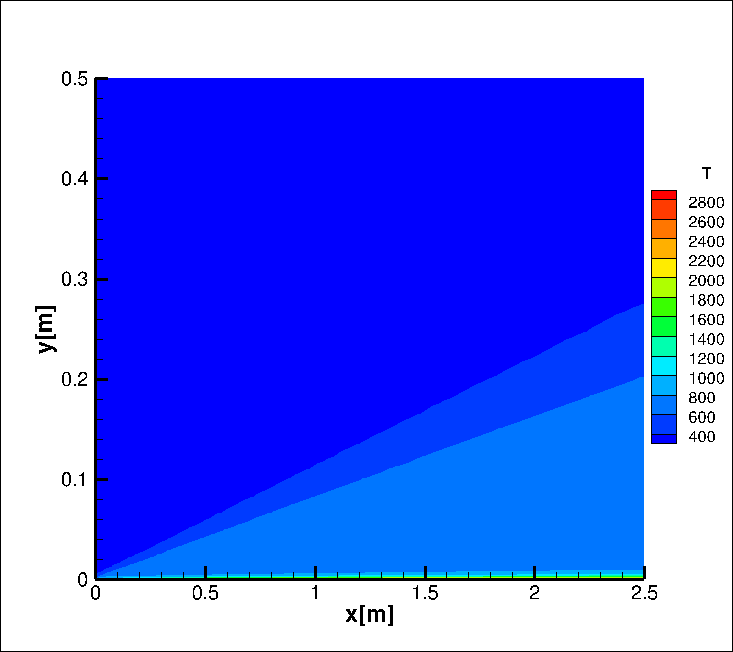
\includegraphics[scale=0.2]{10TempLaminar}
                \caption{Temperature Contour plot}
            \end{subfigure} 
            \begin{subfigure}{0.49\linewidth} \centering 
                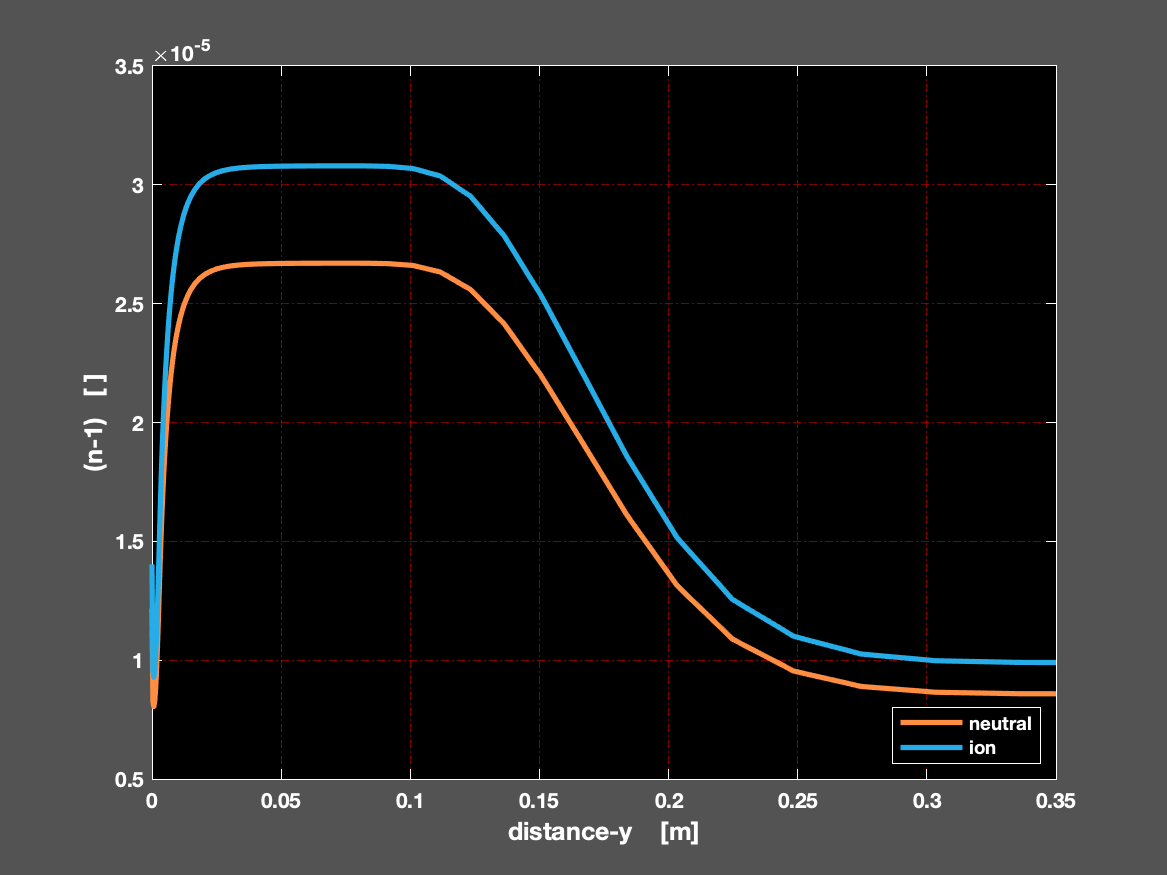
\includegraphics[scale=0.2]{YindexN10Laminar}
                \caption{Index of Refraction on $\hat{y}$ plot}
            \end{subfigure}
        \end{figure}
    \end{frame}
    \begin{frame}{Laminar $\Parenthesis{y=0.1\Units{m}}$}
            \begin{figure}[t]
                \vspace{-1.5cm}
                \centering 
                $$\scriptstyle{ AoA = 10^{\circ},\;\; \Sub{U}{0}=3430\UnitsFrac{m}{s},\;\; \Sub{V}{0}=-605\UnitsFrac{m}{s},\;\;  M = 10.15\Units{\;},\;\; \Sub{\rho}{0} = 3.1\times 10^{-2}\UnitsFrac{kg}{m^3} }$$
            \begin{subfigure}{0.49\linewidth} \centering 
                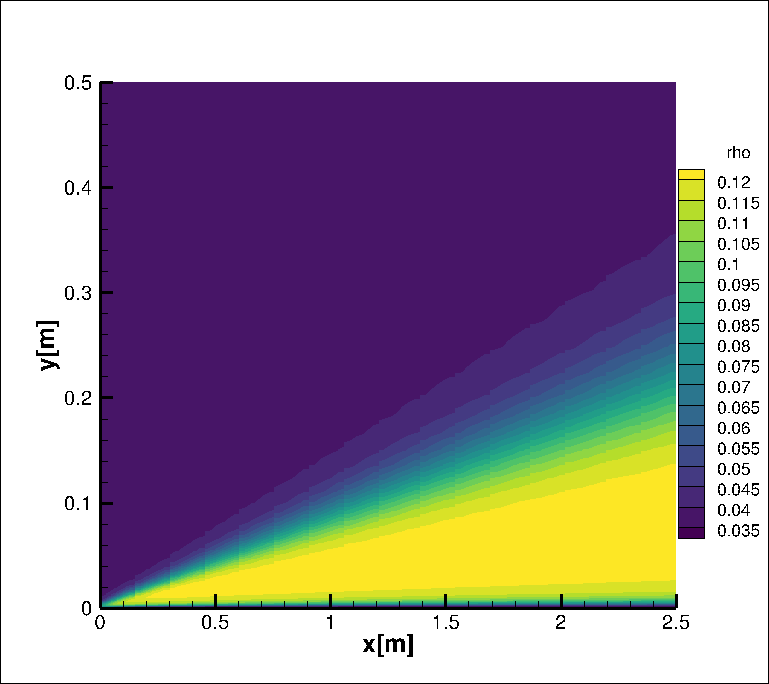
\includegraphics[scale=0.2]{10Laminar}
                \caption{Density Contour plot}
            \end{subfigure} 
            \begin{subfigure}{0.49\linewidth} \centering 
                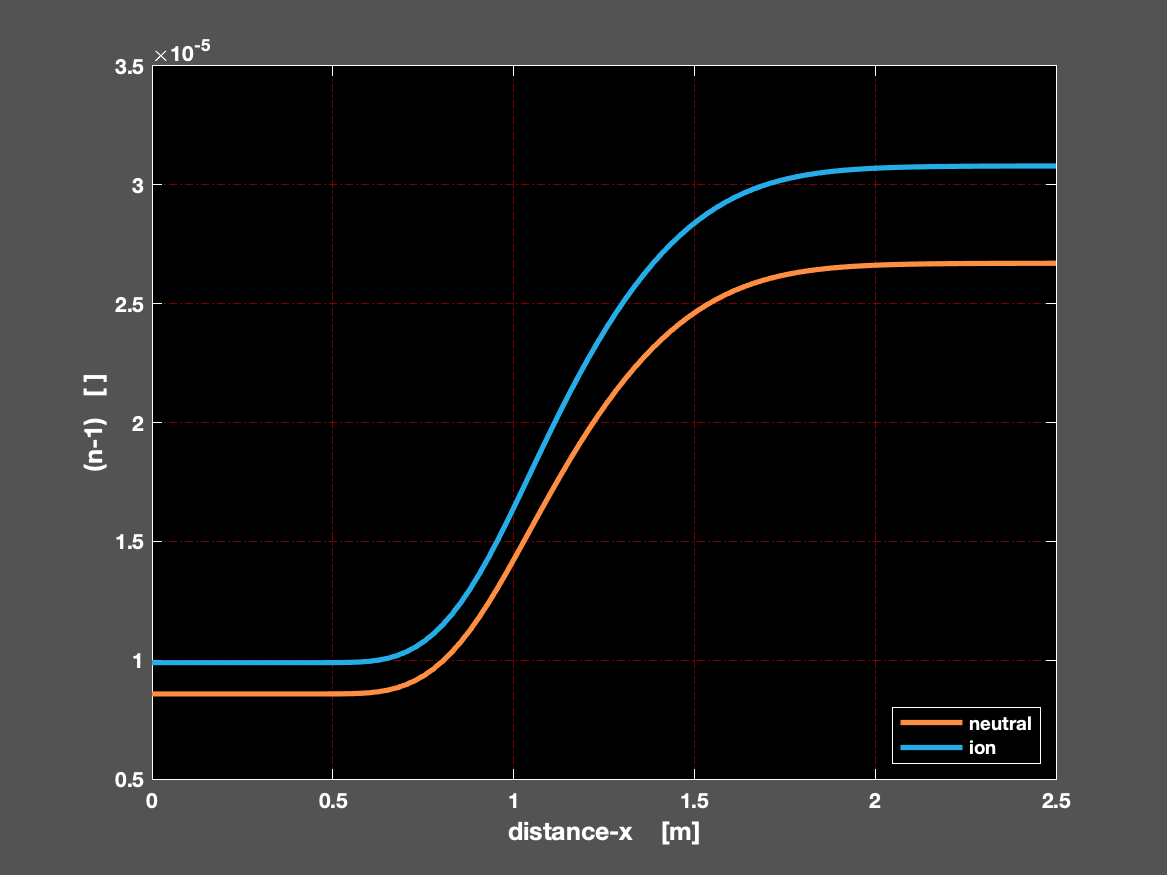
\includegraphics[scale=0.2]{indexN10Laminar}
                \caption{Index of Refraction on $\hat{x}$ plot}
            \end{subfigure}
        \end{figure}
    \end{frame}


    \begin{frame}{Turbulent $\Parenthesis{y=0.1\Units{m}}$}
            \begin{figure}[t]
                \vspace{-1.5cm}
                \centering 
                $$\scriptstyle{ AoA = 10^{\circ},\;\; \Sub{U}{0}=3430\UnitsFrac{m}{s},\;\; \Sub{V}{0}=-605\UnitsFrac{m}{s},\;\;  M = 10.15\Units{\;},\;\; \Sub{\rho}{0} = 3.1\times 10^{-2}\UnitsFrac{kg}{m^3} }$$
            \begin{subfigure}{0.49\linewidth} \centering 
                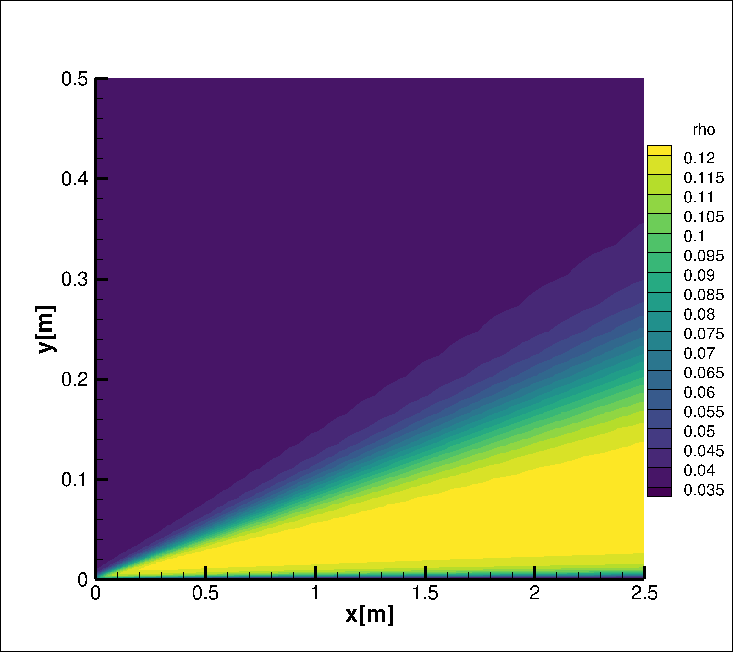
\includegraphics[scale=0.2]{10Turbulent}
                \caption{Density Contour plot}
            \end{subfigure} 
            \begin{subfigure}{0.49\linewidth} \centering 
                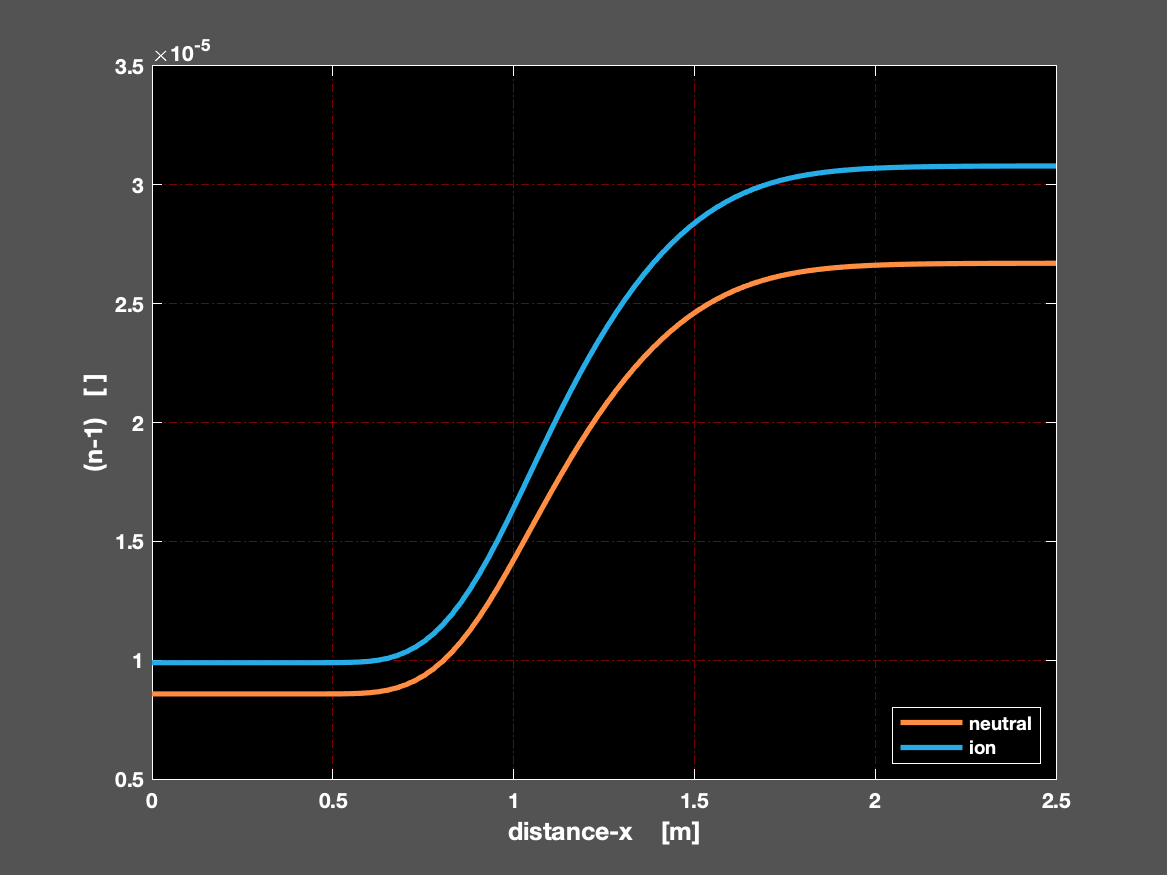
\includegraphics[scale=0.2]{indexN10Turbulent}
                \caption{Index of Refraction on $\hat{x}$ plot}
            \end{subfigure}
        \end{figure}
    \end{frame}


    \begin{frame}{Questions + Discussion}
        \begin{itemize}
            \item Post processing vs. coupled into a CFD model. \\
            \item What kind of discretization is the most appropriate for the optical mesh.\\
            \item How to determine the size of the optical mesh? \\
            \item Mesh Implementation? \\  
            \item What kind of flows and optics characteristics shall we be looking at? \\ 
        \end{itemize}
    \end{frame}
    
\end{document}
